%! TEX root = 'main.tex'
\section{System Setup}
\label{sec:setup}

\subsection{Source Code}

The source code of this 8-bit CPU is uploaded to Github~\footnote{https://github.com/whensungoesdown/8bitcpu}.

It has the following files.

8-bit register:
\begin{itemize}
	\item 8bitreg.bdf
	\item 8bitreg.bsf
\end{itemize}

8-bit ALU:
\begin{itemize}
	\item 8bitalu.bdf
	\item 8bitalu.bsf
\end{itemize}

Control Logic:
\begin{itemize}
	\item controllogic.bdf
	\item controllogic.bsf
	\item controllogicrom.bsf
	\item controllogicrom.cmp
	\item controllogicrom.mif
	\item controllogicrom.qip
	\item controllogicrom.vhd
\end{itemize}

4-bit counter:
\begin{itemize}
	\item counter4b.bdf
	\item counter4b.bsf
\end{itemize}

Memory:
\begin{itemize}
	\item ram16bouten.bdf
	\item ram16bouten.bsf
	\item ram16byte.bsf
	\item ram16byte.cmp
	\item ram16byte.qip
	\item ram16byte.vhd
	\item 16byteram.mif
\end{itemize}

Frequency divider:
\begin{itemize}
	\item clk1MHz.bsf
	\item clk\_div50.vhd
\end{itemize}


CPU assembly:
\begin{itemize}
	\item testcpu3.bdf
	\item testcpu3.qpf
	\item testcpu3.qsf
\end{itemize}

Waveform files for debugging purpose:
\begin{itemize}
	\item *.vwf
\end{itemize}


\subsection{Setup}
The FPGA developing board we use is Cyclone II EP2C5 Mini Dev Board~\cite{cyclone2}. And the software we use is Quartus II 64-bit Web Edition.

The display we use is 1602A LCD. The hardware setup is shown in~\autoref{fig:setup}.


\begin{figure}[th]
	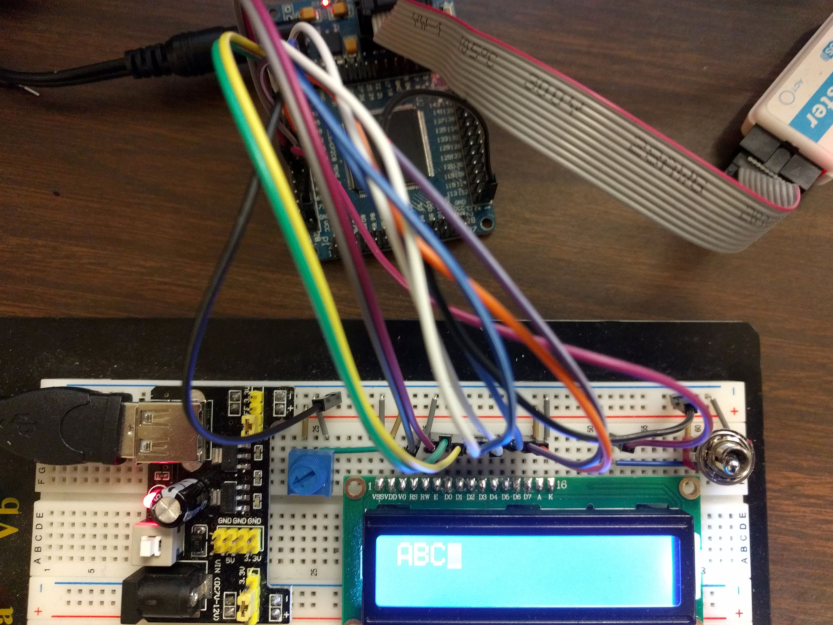
\includegraphics[width=0.47\textwidth]{figures/setup}
	\centering
	\caption{The CPU and display setup.}
	\label{fig:setup}
\end{figure}

We also need a USB Blaster to download the compiled code to the development board.

Both the Cyclone II development board and the LCD need 5V power supply. We power them separately with common ground. The FPGA's GPIO operating voltage is 3.3V. Because the LCD data pins have a wide range of operating voltage which accept 3.3V signals, we can directly connect the GPIO on the FPGA to the LCD. 
